This chapter introduces and explains the fundamentals to understand the rest of the this disseration. Related work is also reviewed and directly compared against the proposed project.

\section{Fundamentals on \acl*{SLAM} (\acs*{SLAM})}

From the beginning of civilization, mapping the surroundings has been a key concept for navigating the environment. In essence we faced the same problem as our ancestors: How do we map the environment and know our location within it? \acs*{SLAM} is the challenge of mapping the local environment of a moving entity (e.g. robot) and updating the map continuously as the entity moves through space. This is a massive problem to tackle on and of extreme importance to achieve robot autonomy. A robot's autonomy is based on its understanding of its surrounding environment, which can be obtained through sensors. There are many types of sensors that are useful for this purpose, sensors such as:
\textcolor{red}{EXPLAIN THESE SENSORS}
\begin{itemize}
    \item \acs*{LiDAR}
    \item RGB-D cameras
    \item \acs*{IMU}
    \item \acs*{GPS}
\end{itemize}

\acs*{SLAM} could technically be split into two segments, one that is mapping and the other localization. Although it is possible to know the localization without knowledge of the map, there will always be some localization information needed when mapping an environment, unless the entity has a fixed position.

\subsection{Localization}
Localization can take two forms: relative or global. Relative localization, as the name suggests, creates a relation between two different poses (position and orientation). A pose's current state is usually determined by its last state. Information provided by global localization can be viewed independently of other positions.

To compute relative localization it is common to use data from motion sensors, such as wheel encoders and \acs*{IMU}s, to estimate change in pose over time.


\todo[inline]{Talk about odometry, Visual odometry algorithms? ICP?}



Many times sensor information is to noisy to be directly use as an input, which is a problem. A common way to solve this problem is to use a Kalman filter.

\subsubsection{Kalman Filter}
The Kalman filter is a linear iterative process, as shown in Fig. \ref*{fig: flowchart kalman}, that uses consecutive data input to quickly converge to the true value. Each iteration involves computing three values: the Kalman gain, the current estimate, and its uncertainty. The Kalman gain uses the previous uncertainty and the error in data. The estimate of the current iteration is computed with the new data input and the previous estimation, where the weight of each component is decided by the kalman gain. Once the current estimate has been calculated, the new uncertainty of the estimate is computed with the current estimate and kalman gain.

\begin{figure}[H]
    \centering
    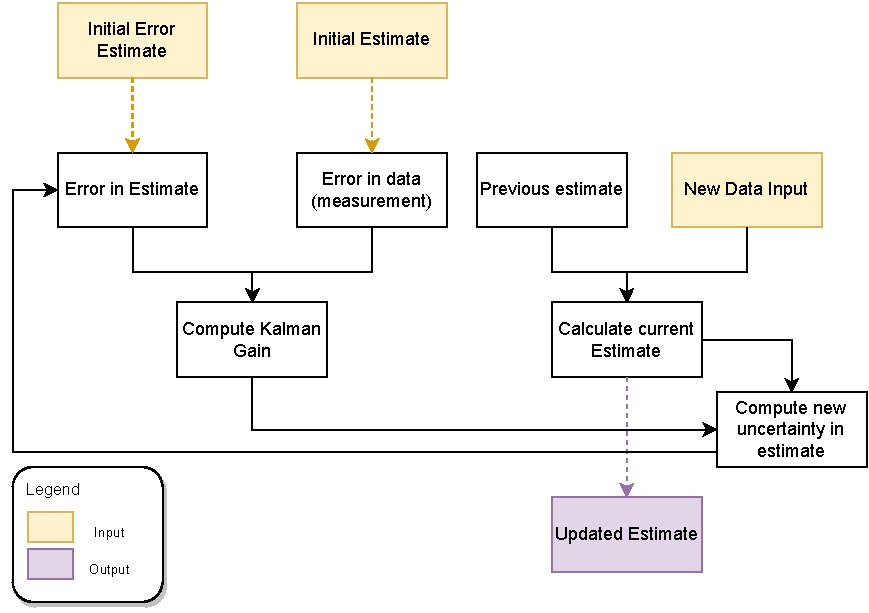
\includegraphics[width=0.7\linewidth]{images/background/Kalman-diagram.pdf}
    \caption{Simple flowchart of the Kalman Filter. \textcolor{red}{ADD REFERENCE}}
    \label{fig: flowchart kalman}
\end{figure}


In real world it is uncommon to have a global linear system and due to it's linearity, the Kalman Filter won't work well in non-linear scenarious. A simple way to solve this is to make the global nonlinear function, locally linear, using a first order Taylor Expansion to do the aproximation. This is what the method the \acl{EKF} \acs*{EKF} deploy.


 A more accurate way to solve the problem is to use a \acl*{UKF} (\acs*{UKF}).

 \subsection{Mapping}

\subsection{Loop Closure}

\subsection{Moving Objects}

\section{\acs{ROS}}

An effective robotics project cannot be achieved by just having sensors and physical components; rather, one must have a clever communication system between sensors and processes. Although such complex systems can be built from scratch, it is not worthwhile when software like \acs*{ROS} is available.

Although the name \acl*{ROS} suggests that ROS is an operating system, this is not the case.  In a way, \acs*{ROS} is both middleware and a framework. The system provides a communication channel where messages can be easily subscribed, published and distributed, allowing quick integration between systems and components. Moreover, it provides features such as debugging, visualization, testing, logging, and configuration right out of the box. Additionally, ROS includes a number of useful packages for essential areas relevant to robotics such as movement, perception, and manipulation. The ROS community is also constantly evolving with the most recent developments in robotics, so libraries are always being added to ROS. In robotics, it is considered the standard platform for developing complex projects.


\section{Data Acquisition Apparatus}

It is no surprise that there are already a number of portable and light sensors designed to collect sensor data about the environment around us. There are several proprietary solutions available on the market for gathering sensory information for \acs*{SLAM}, but they tend to be expensive \cite{libackpack_C50}, \cite{libackpack_DGC50}. Additionally, there are some articles and research papers that have been conducted with the goal of building a system similar to the one proposed here. These works will be the ones to be focused on since the methodology, and results are readily available.

In terms of application, Alexander Proudman's system is closest to this project's \cite{proudman_online_2021}. Based on an Ouster OS0-128 \acs{LiDAR} and a RealSense D435i, both with an integrated \acs{IMU}, the system performs online \acs{SLAM} and estimates \acl{DBH} (\acs*{DBH}) using the data collected. While their application has the benefit of having a built-in display that allows real-time visualization of data, one of its major drawbacks is the way they build their apparatus, opting for a metal stick rather than a backpack type of design. As the authors acknowledge, user fatigue may lead to excessive variations in stick position, resulting in unintelligible and uncontrolled movements, damaging the performance of the apparatus.This would not be an issue if a more ergonomic structure was used. The errors due to user fatigue can be a slightly mitigated by performing \acs{SLAM} in several sessions instead of one, allowing the user to rest between shorter sessions \textcolor{red}{INSERT REFERENCE TO THE SECOND PAPER}. After recording multiple sessions, \acs*{GPS} information is used to assemble the multiple sessions's map into a single map.

Recently, Kui Xao developed a dual \acs*{LiDAR}s system, an \acs*{IMU}, and \acs*{GPS} for performing \acs*{SLAM} in multi-scene applications \cite{xiao_high-precision_2022}. To increase the vertical \acl*{FOV} (\acs*{FOV}), one of the \acs*{LiDAR}s was placed in the \textit{XY} plane while the other was positioned at -77.94° from the \textit{XY} plane. A timestamp synchronization algorithm is used by the authors to merge the data of the two \acs*{LiDAR}s. Secondly, the \acs*{LiDAR} data is tightly coupled with the IMU data in order to reduce noise caused by the inaccuracy of \acs*{LiDAR}-based odometry. In outdoor tests, the \acs*{IMU} calibration is improved by loosely coupling \acs*{GPS} to the \acs*{IMU} during outdoor tests.